\documentclass[compress,blue]{beamer}
\logo{\includegraphics[width=0.12\textwidth]{stout_logo}\hspace{-2pt}}
% \usetheme{default}
%\usetheme{Boadilla}
%\usetheme{Bergen}
\usetheme{Berkeley}
%\usetheme{Goettingen}
%\usetheme{Hannover}
%\usetheme{Luebeck}
% \usetheme{Madrid}
%\usetheme{Montpellier}
%\usetheme{Rochester}
%\usetheme{Warsaw}

% \mode<presentation>
\usepackage{amsmath} \usepackage{graphicx}
\usepackage{amsfonts} \usepackage{amssymb}

\def\QED{{\ \vbox{\hrule\hbox{\vrule height1.3ex\hskip0.8ex\vrule}\hrule}}\par}
\def\ds{\displaystyle}
\newcommand{\pdiff}[2]{\frac{\partial #1}{\partial #2}}
\newcommand{\pdiffsec}[2]{\frac{\partial^2 #1}{\partial^2 #2}}
\newcommand{\diff}[2]{\frac{d #1}{d #2}}

%%%%%%%%%%%%%%% EITHER DEVELOP A CATCHY TITLE OR USE THE INDUSTRY SPONSOR NAME %%%%%%%%%%%%%%%
\title{The District Company}
%%%%%%%%%%%%%%% IF THE COMPANY NAME DOES NOT APPEAR, PLACE IT AFTER THE LIASON'S NAME %%%%%%%%%%%%%%%
%%%%%%%%%%%%%%% E.G. Steve Jobs, Apple Inc. %%%%%%%%%%%%%%%
\subtitle{Industry Liason: Dustin Jepperson}

%%%%%%%%%%%%%%% ENTER YOUR GROUP MEMBERS HERE %%%%%%%%%%%%%%%
\author{Megan Mortensen, Connor Phu, \\
Brian Dassow, Bella Nordahl}

%%%%%%%%%%%%%%% REPLACE THE BLUE DEVILS LOGO WITH THE COMPANY LOGO IF ONE EXISTS %%%%%%%%%%%%%%%
\titlegraphic{\includegraphics[width=0.33\textwidth]{pic_math_logo}\hspace{0cm}
\includegraphics[width=0.33\textwidth]{DistrictCompanylogo}}

\institute{\textbf{University of Wisconsin-Stout} \\
}
\date{March 10, 2016}

\begin{document}

% this prints title, author etc. info from above
\frame{\titlepage}

%\frame{\frametitle{Outline}\tableofcontents[pausesections]}

%%%%%%%%%%%%%%% BELOW IS YOUR SLIDE DECK %%%%%%%%%%%%%%%
%%%%%%%%%%%%%%% CHANGE SLIDE TITLES, ETC. AS YOU DEEM APPROPRIATE %%%%%%%%%%%%%%%
%%%%%%%%%%%%%%%%%%%%%%%%%%%%%%%%%%%%%%%%%%%%%%%%%%%%%%%%%%%
%%%%%%%%%%%%%%% MUST INCLUDE:
%%%%%%%%%%%%%%% (1) Give a statement of the problem and tell why the problem is important
%%%%%%%%%%%%%%% (2) Brief statement of your results
%%%%%%%%%%%%%%% (3) Details about your approach to the problem  
%%%%%%%%%%%%%%% (4) More detailed presentation of your results
%%%%%%%%%%%%%%% (5) Restatement of the problem and the results
%%%%%%%%%%%%%%% (6) Suggested future work
%%%%%%%%%%%%%%% (7) Acknowledgements slide (Leave this slide in the deck, just edit accordingly.)
%%%%%%%%%%%%%%% %%%%%%%%%%%%%%% %%%%%%%%%%%%%%% %%%%%%%%%%%%%%%


\section{Action Plan}

\begin{frame}{Action Plan}
\setbeamertemplate{itemize items}[circle]
\begin{itemize}
  \item Use regression to look at correlation between events and concession
  sales
  \item Use classifiers to determine what would help the company based on survey
  responses and Facebook reviews
\end{itemize}
\end{frame}

\section{Facebook Reviews}

\begin{frame}{Facebook Reviews}
\setbeamertemplate{itemize items}[circle]
\begin{itemize}
  \item 
\end{itemize}
\end{frame}

\section{Survey}

\begin{frame}{Survey}
\vspace{-.6cm}\hspace{9.5cm}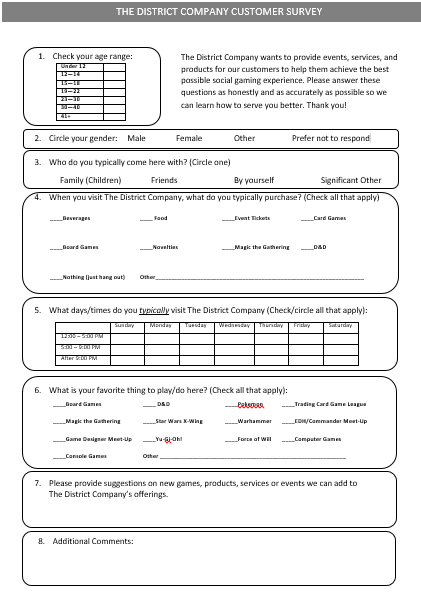
\includegraphics[width=.6\textwidth]{DistrictSurvey}
\end{frame}

\section{Data Analysis}


\begin{frame}{Correlations}
\begin{rows}
\row{\textwidth}
\centering
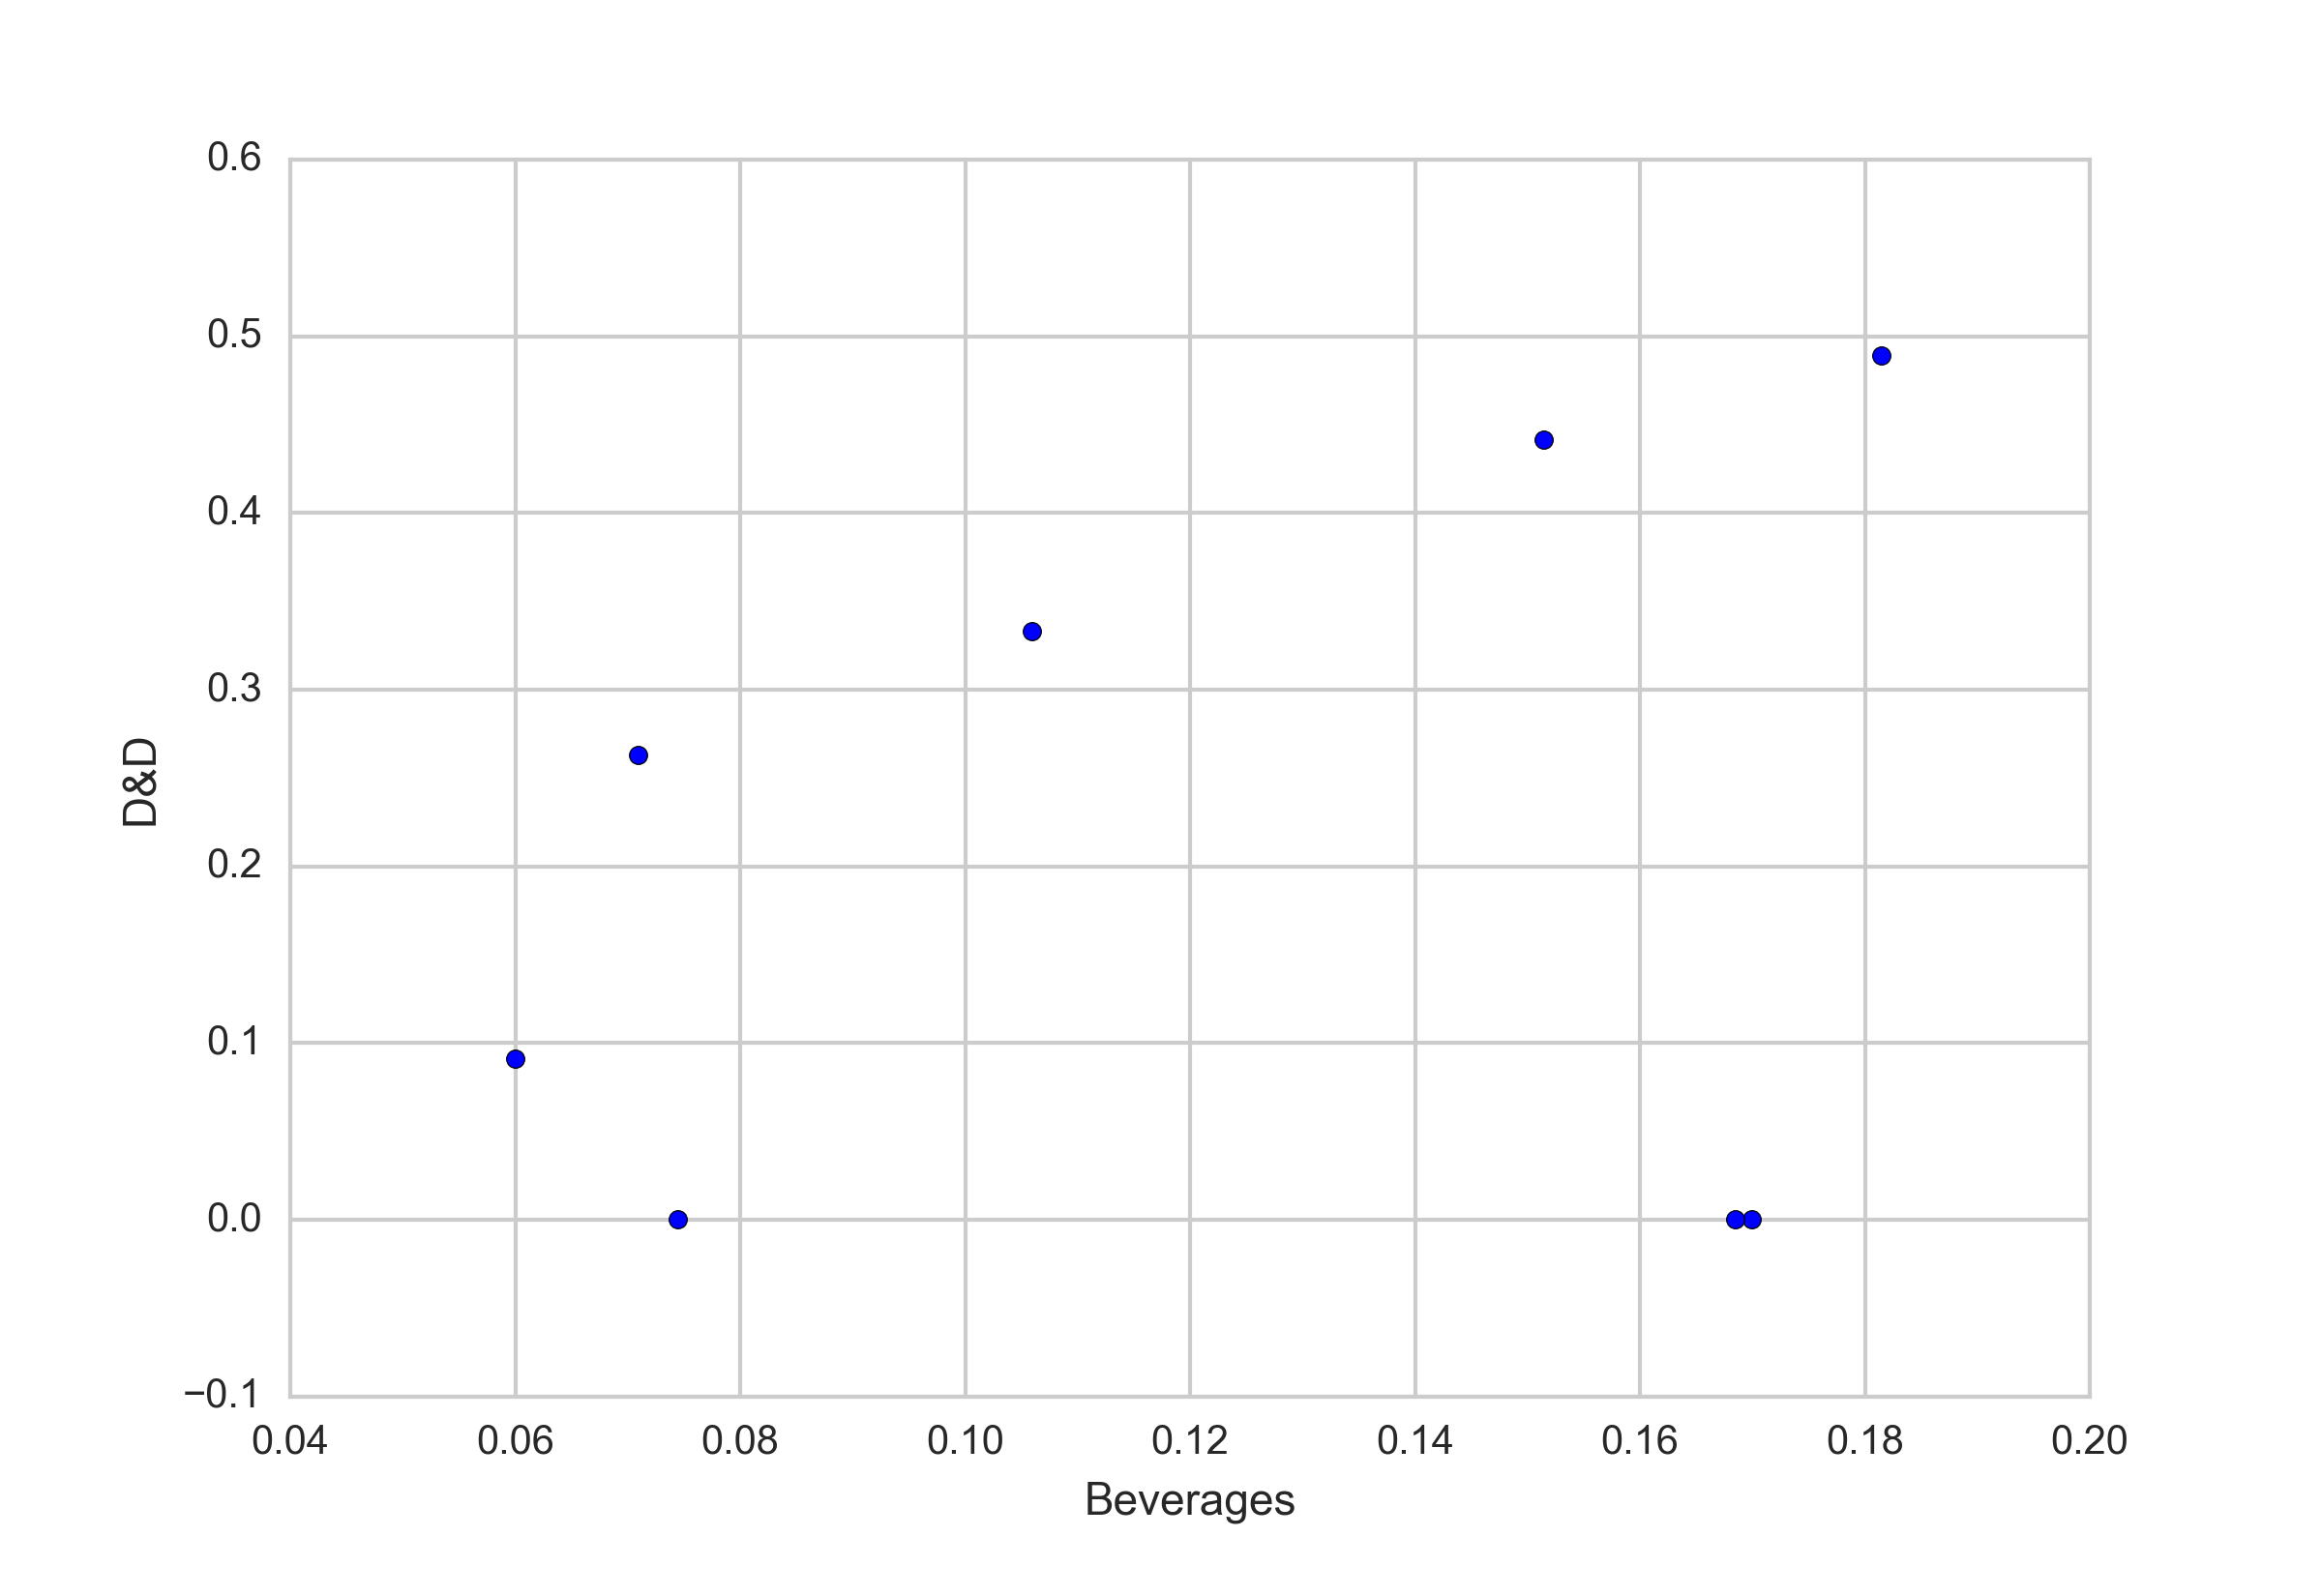
\includegraphics[width=5cm,height=4cm]{DandD_Beverages}
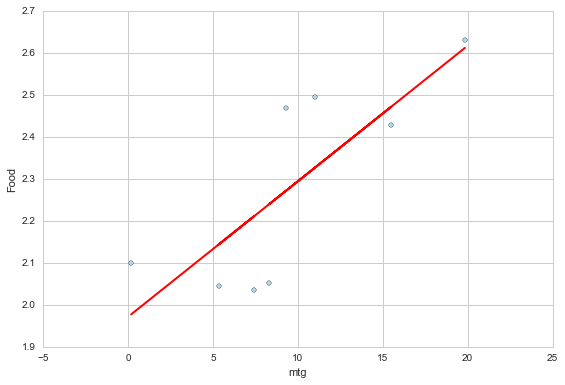
\includegraphics[width=5cm,height=4cm]{mtg_food}
\row{\textwidth}
\centering
\hspace*{2.5cm}
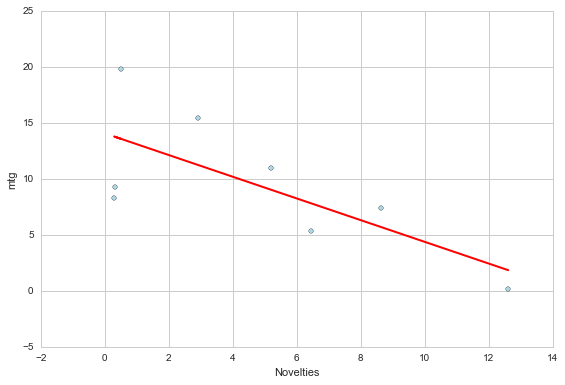
\includegraphics[width=5cm,height=3.75cm]{mtg_novelties}
\end{rows}
\end{frame}

\begin{frame}{Monthly Totals}
\vspace{-.6cm}\hspace{9.5cm}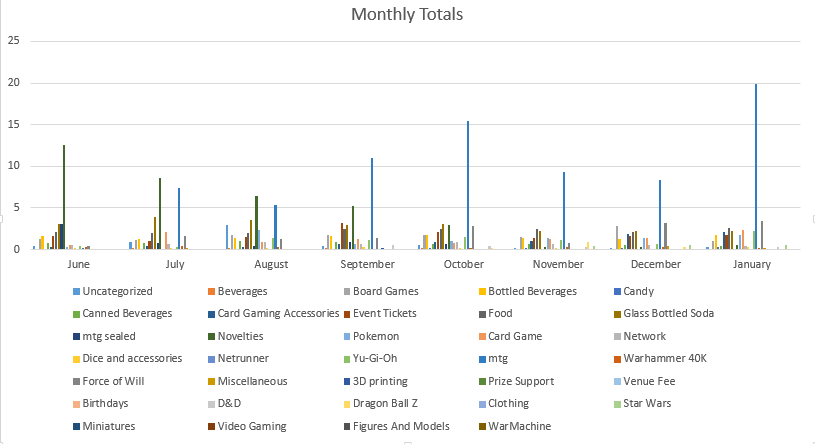
\includegraphics[width=1\textwidth]{monthlyTotals}
\end{frame}

\begin{frame}{Monthly Data Continued}
\begin{rows}
\row{\textwidth}
\centering
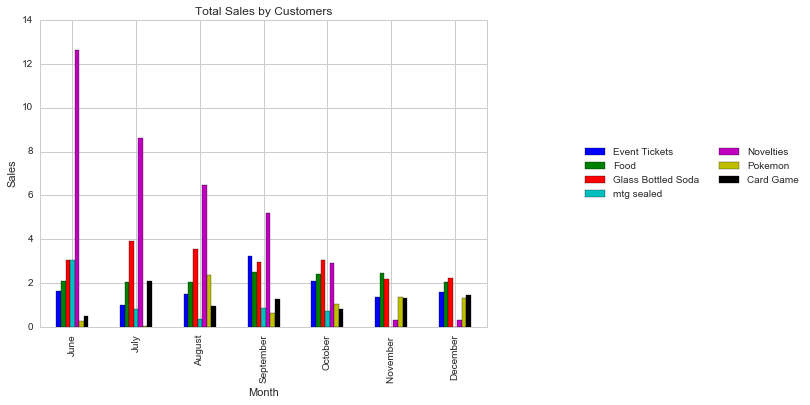
\includegraphics[width=5cm,height=4cm]{SalesByMonth1}
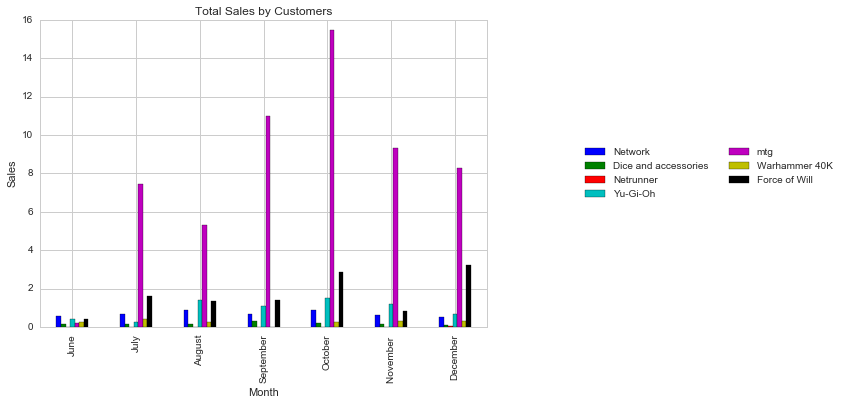
\includegraphics[width=5cm,height=4cm]{SalesByMonth2}
\row{\textwidth}
\centering
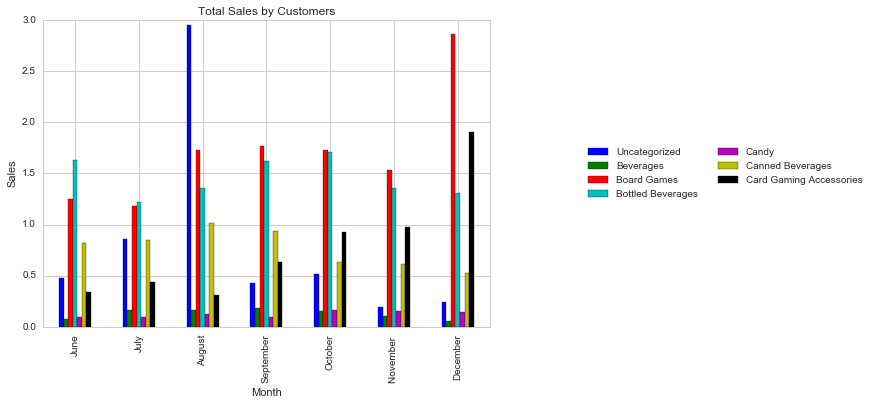
\includegraphics[width=5cm,height=4cm]{SalesByMonth3}
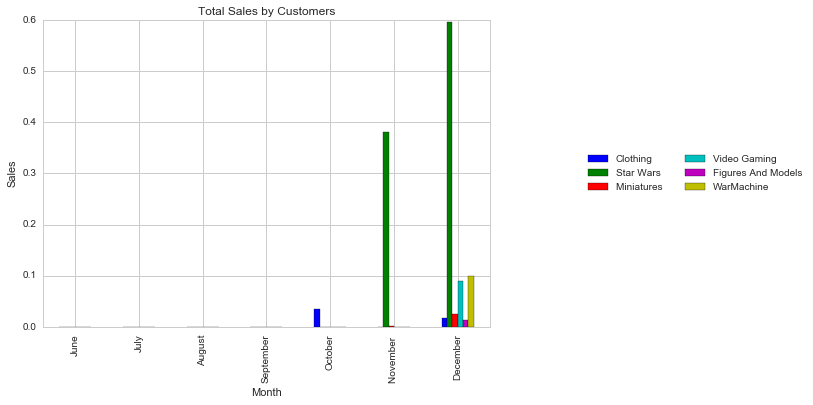
\includegraphics[width=5cm,height=4cm]{SalesByMonth4}
\end{rows}
\end{frame}

\begin{frame}{Weekly Data}
\begin{rows}
\row{\textwidth}
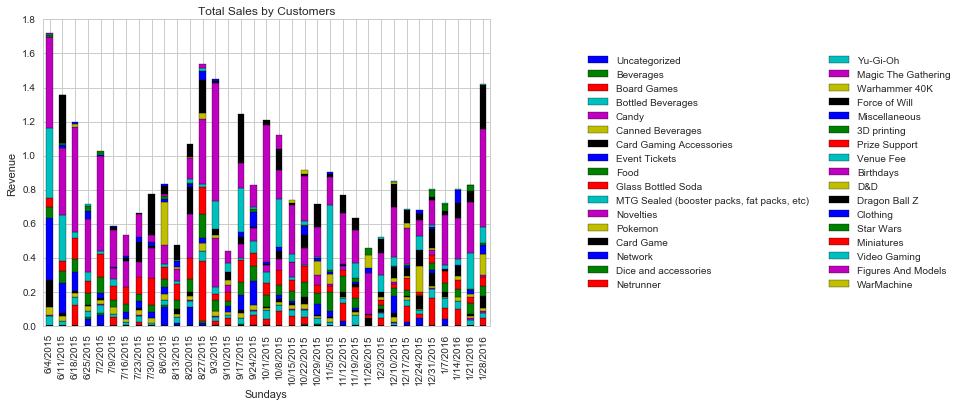
\includegraphics[width=3.5cm,height=2.5cm]{RevenueSundays}
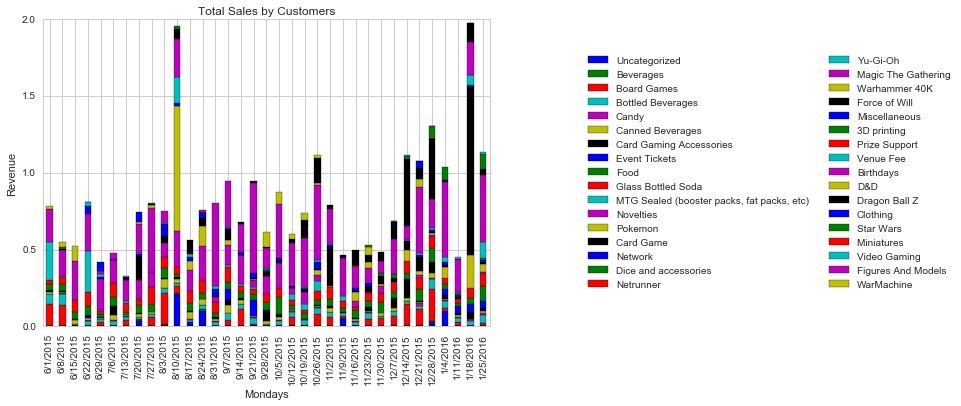
\includegraphics[width=3.5cm,height=2.5cm]{RevenueMondays}
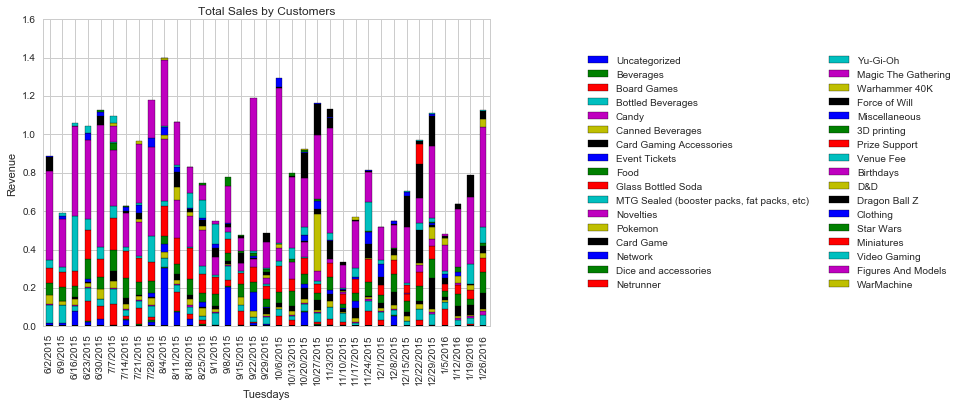
\includegraphics[width=3.5cm,height=2.5cm]{RevenueTuesdays}
\row{\textwidth}
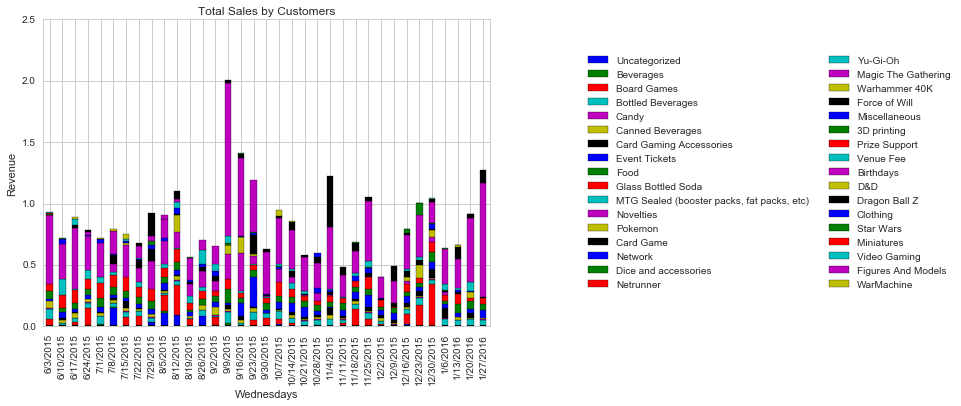
\includegraphics[width=3.5cm,height=2.5cm]{RevenueWednesdays}
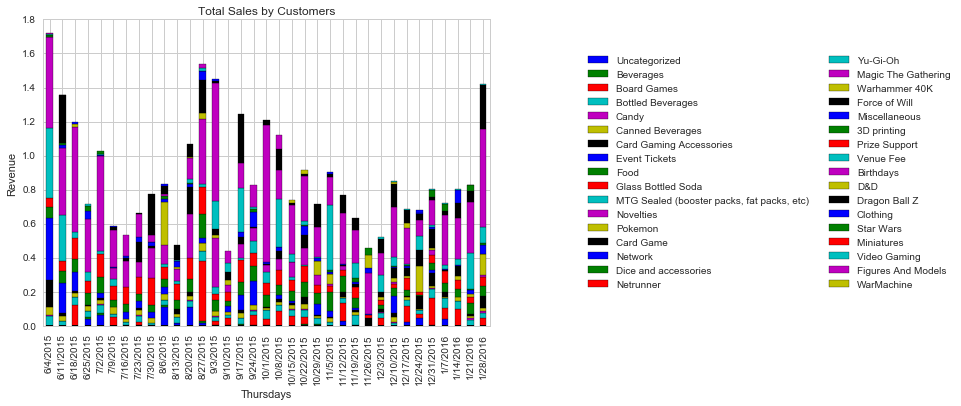
\includegraphics[width=3.5cm,height=2.5cm]{RevenueThursdays}
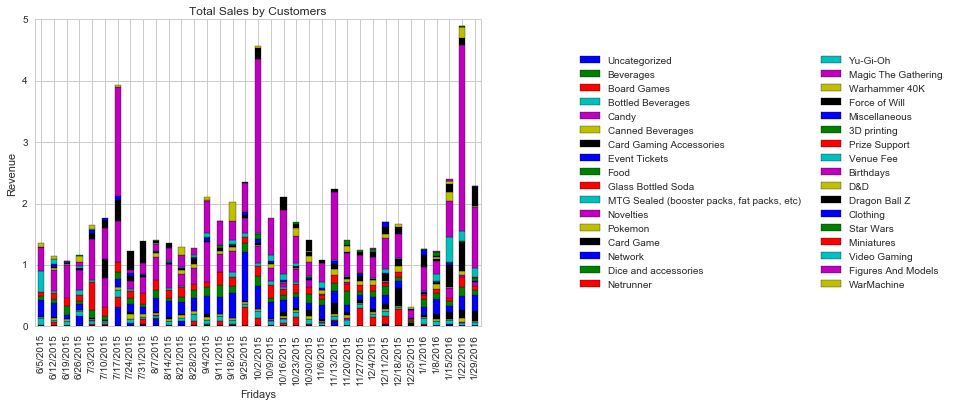
\includegraphics[width=3.5cm,height=2.5cm]{RevenueFridays}
\row{\textwidth}
\hspace*{3.45cm}
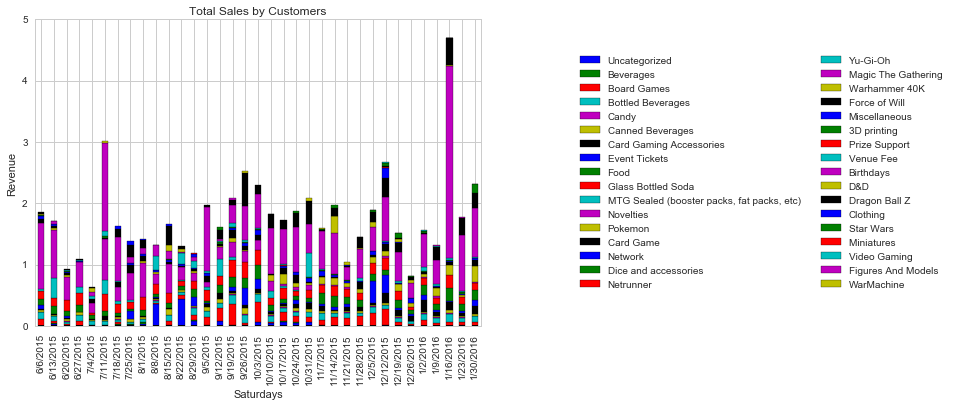
\includegraphics[width=3.5cm,height=2.5cm]{RevenueSaturdays}
\end{rows}
\end{frame}


\end{document} 
